\documentclass[12pt,a4paper]{article}
\usepackage[margin=3cm,bottom=3cm]{geometry}
\usepackage[utf8]{inputenc}
\usepackage{hyperref}
\usepackage{graphicx}
\usepackage[table]{xcolor}
%page anchorlar gerekirse alt satırı sil
\hypersetup{pageanchor=false}
\usepackage[document]{ragged2e}
\usepackage[T1]{fontenc}


\begin{document}
\begin{titlepage}
 \centering
 
\includegraphics[scale=0.3]{bilgi_logo}\\
 
 {\scshape\Large Department of Computer Engineering\\}
 {\scshape\Large Faculty of Engineering and Natural Sciences\\}
 \vspace{3cm}
 {\huge\bfseries BASTION THE SENTINEL\\}
 {\scshape\Large Park Cleaner Robot\\}
 \vspace{4cm}
 {\Large\itshape Furkan Karakoyunlu\\}
 {\Large\itshape 112200036\\}
 \vspace{4cm}
 {\Large\itshape Supervised by\\Eray Baran}
 \vfill
 \vfill
 {\large \today\\}
 \href{http://www.bastionthesentinel.com}{www.bastionthesentinel.com}
\end{titlepage}


% Table of contents
\tableofcontents
\pagebreak
\listoffigures
\pagebreak

\section{Abstract}
\justify
In today’s era consuming is essential for human beings. We consume more than we produce. This “consuming” leads to 
waste which is a danger for Mother Nature. It leaves a great amount of damage to the nature. Thus, there is huge space 
to fill for recycling and Bastion the Sentinel will help to close the gap. We are aiming for people to not waste their 
time for garbage collecting and separating for recycling from the beginning. The purpose of creating this robot is 
reducing manpower in collecting garbage and increase recycling to make future better. 
\begin{figure}[h!]
  \begin{center}
    
\includegraphics[scale=0.4]{bastion}
    \caption{Bastion The Sentinel}
  \end{center}
\end{figure}

\section{Device Functionality and Overall Design}
Bastion the Sentinel is designed as a semi-autonomous robot. It will be a multi-tasking robot and it has two main parts. 
First part is movement controls and the second part is collecting garbage via image-processing. In addition to image processing 
abilities it can also be controlled by an operator. In the image processing part, it will consider color and it will recognize 
red, blue, yellow colors. It will separate all of the garbage by particularly and put them into box which is placed on top of 
the robot. After that operator will do separation. If there are one or more objects to collect, operator can change the box’s 
volume and decide the count of separators. There could be obstacles around or unfavourable weather conditions like rain, snow, 
etc. Therefore, some incidents are inevitable. Because of this top of the box can be closable.

Bastion the Sentinel has six wheels driving him. The wheels rotating to accelerate the Bastion the Sentinel, the wheels 
are not rotating to change the rotation of the Bastion the Sentinel. The rotation changes by rotating the wheels in a 
different speeds and/or directions. For example the wheels on the left hand side are rotating forwards with a speed of 
1 km/h and the wheels on the right hand side are rotating backwards with a speed of 1 km/h; Bastion the Sentinel will 
be turning right in the same place. 
There are six DC motors to rotate the six wheels. The DC motors’ speed are adjustable. Bastion the Sentinel has three different speed presets. 

\section{Hardware}
\subsection{Raspberry Pi 3}
The Raspberry Pi is a small sized computer that can be plugged to TV or other external display and can operate as Linux machine. 
It is widely used for electronic projects and many other things that our laptops or desktop computers does. It can also record and 
play high-definition videos.

Image processing is a really hard work that can’t be done with simple tools, it needs a good processor and transaction memory. 
Thus, Raspberry Pi 3 is a great tool for this kind of projects.
\begin{figure}[h!]
  \begin{center}
    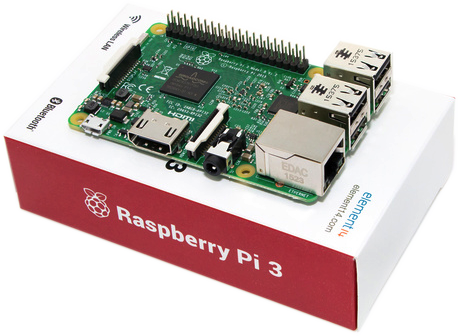
\includegraphics[scale=0.5]{pi_box}
    \caption{Raspberry Pi 3 with box}
  \end{center}
\end{figure}

\subsection{Raspberry Pi 3 Camera Module v1.3}
All the visual data will be gathered by this camera module. The module can also be used for to take high definition videos and photographs. 
In order to reduce the workload on processors and to speed up image processing, in this project our streaming dimensions are 640 pixel wide 
and 480 pixel high.

The Raspberry Pi 3 will be streaming video to server and all image processing part will be done on server.
\begin{figure}[h!]
  \begin{center}
    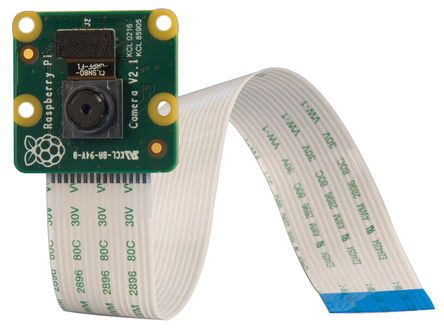
\includegraphics[scale=0.3]{pi_camera}
    \caption{Raspberry Pi camera module}
  \end{center}
\end{figure}

\subsubsection{Image Processing}
Image processing is a method to perform some operations on an image, in order to get an enhanced image or to extract some useful 
information from it. It is a type of signal processing in which input is an image and output may be image or characteristics/features 
associated with that image. Nowadays, image processing is among rapidly growing technologies. It forms core research area within engineering 
and computer science disciplines too.

Image processing basically includes the following three steps:
\begin{itemize}
 \item Importing the image via image acquisition tools
 \item Analyzing and manipulating the image
 \item Output in which result can be altered image or report that is based on image analysis.
\end{itemize}

There are two types of methods used for image processing namely, analogue and digital image processing. Analogue image processing can be 
used for the hard copies like printouts and photographs. Image analysts use various fundamentals of interpretation while using these visual 
techniques. Digital image processing techniques help in manipulation of the digital images by using computers. The three general phases that 
all types of data have to undergo while using digital technique are pre-processing, enhancement, and display, information extraction. 

In our project we used OpenCV and Raspberry Pi 3 for image processing. To access our image data we are using socketserver and http libraries on 
python3. Basically Raspberry Pi 3 serves video data to http over the wifi and we are capturing that data on the server side. In order to reduce 
the workload on the Raspberry Pi, we are processing our image data on a server. Our process steps as follow:
\begin{itemize}
 \item Start \verb|stream.py| script on Raspberry Pi to stream on http.
 \item Run \verb|colorTracking.py| python script on the server side.
\end{itemize}

As a result of these operations, we able to see a window on server machine that tracks the given color ranges such as red, blue, yellow.

\pagebreak
\subsection{Arduino Mega}
Arduino is an open source electronics platform. It has a programmable microprocessor and it has an interface which makes it easier to program. 
It has 54 digital input/output pins (14 can be used as PWM outputs), 16 analog inputs. In this project the needed pin number is really 
high because of that arduino mega is suitable for this project. 
\begin{figure}[h!]
  \begin{center}
    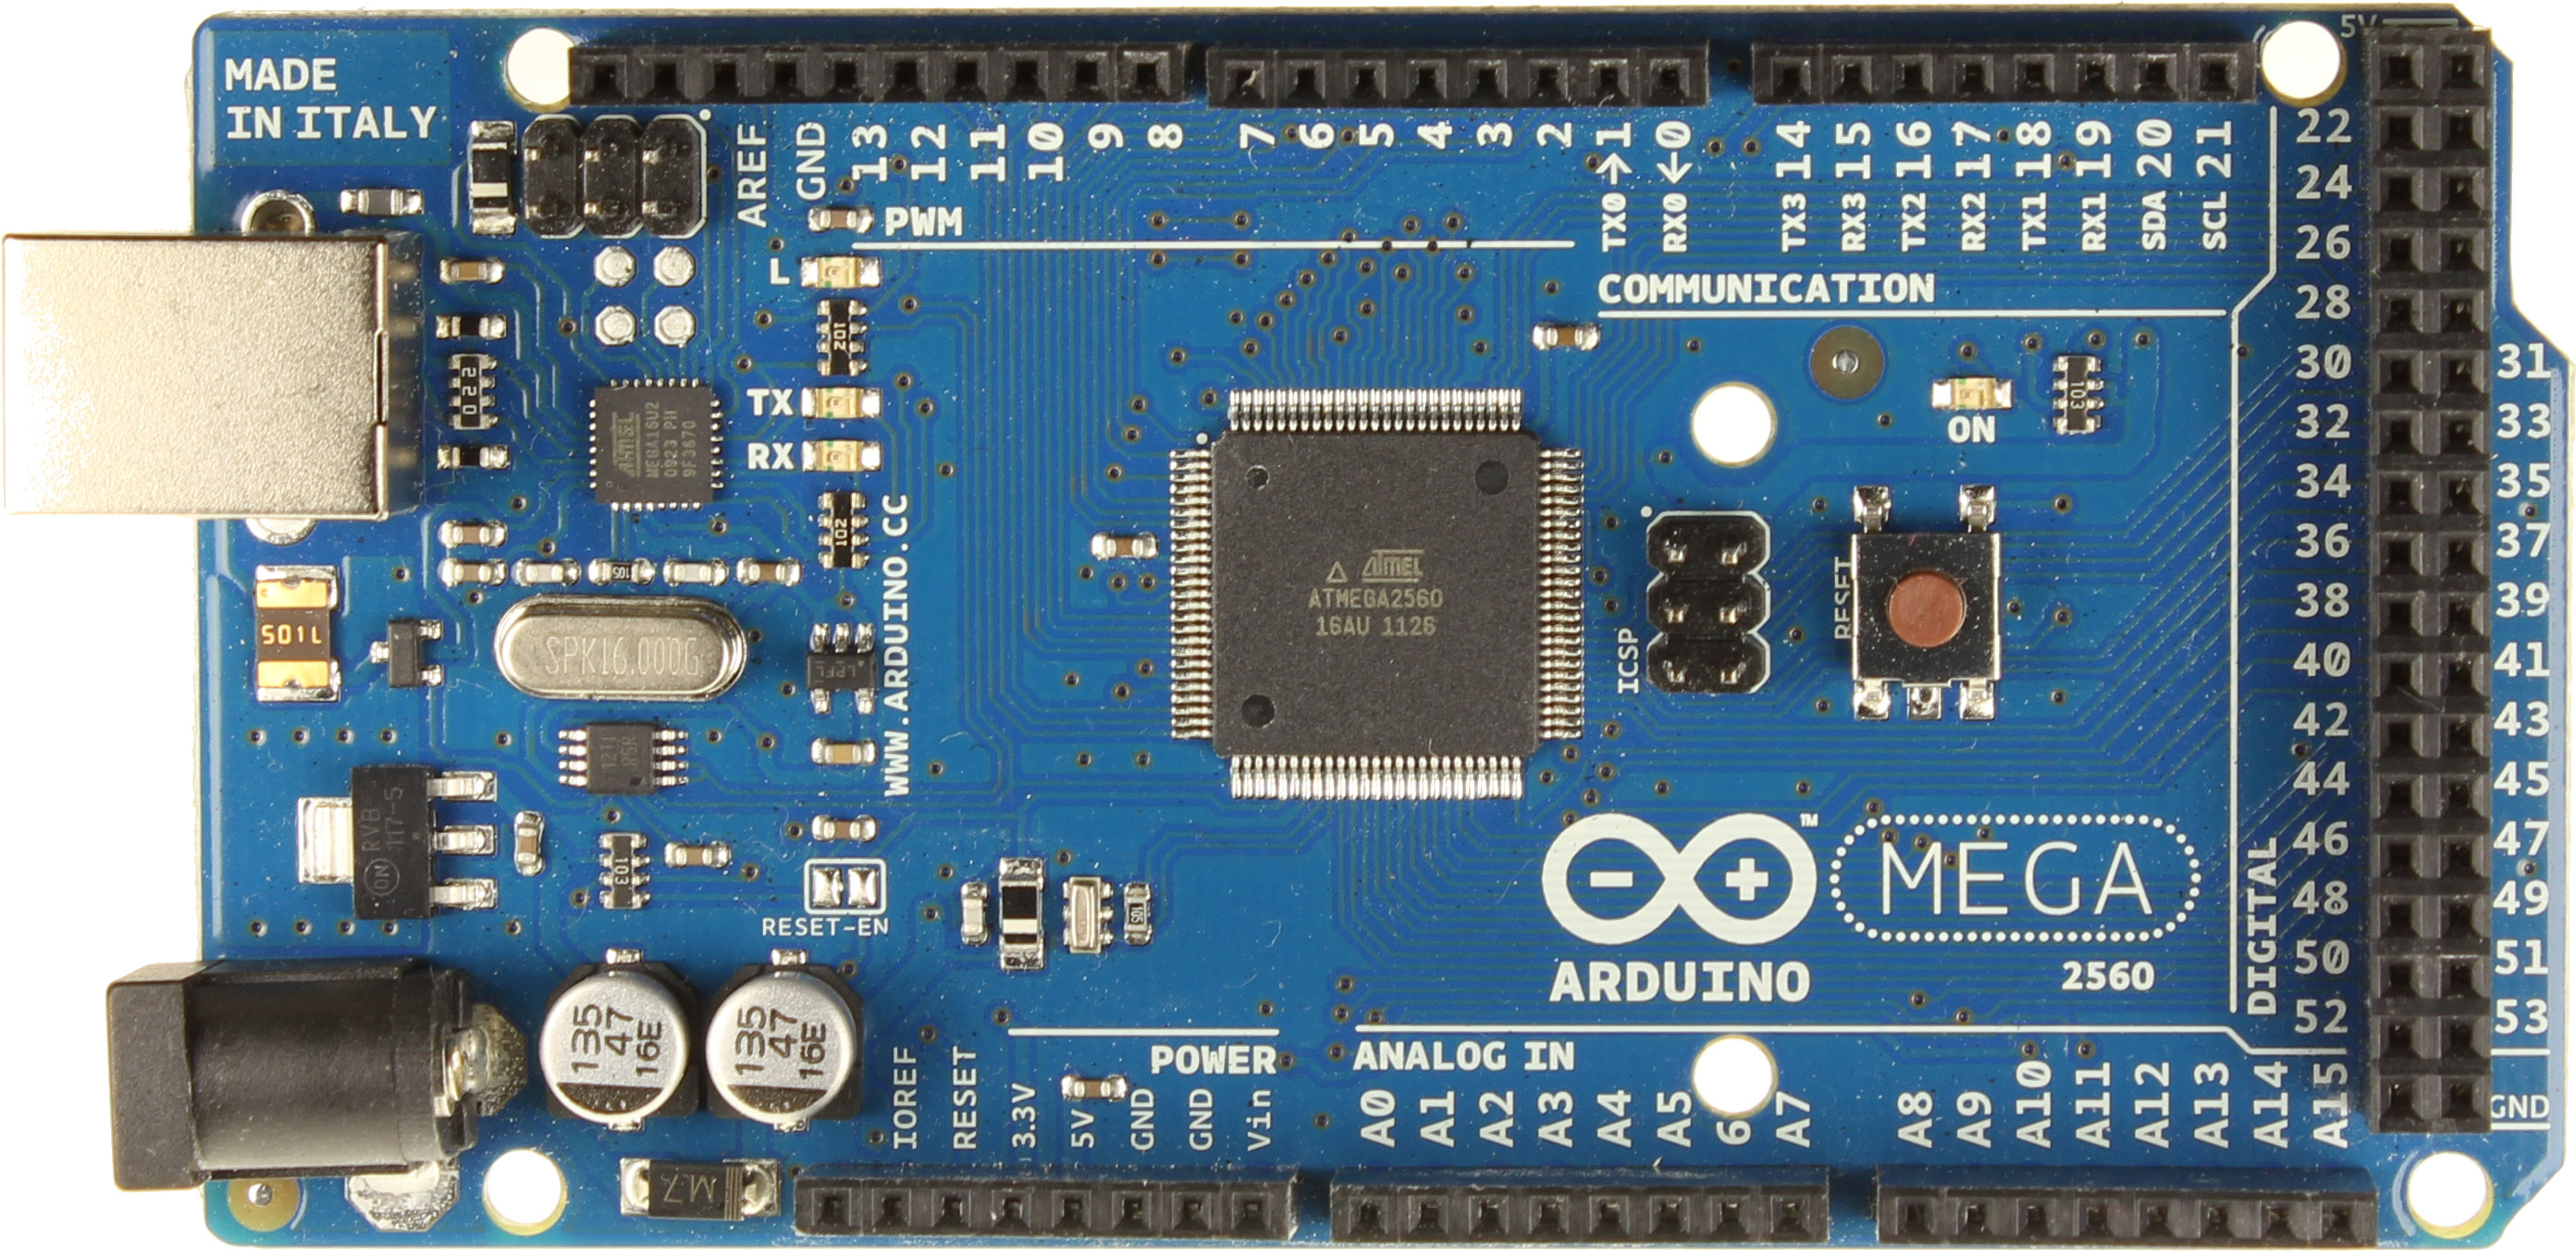
\includegraphics[scale=0.1]{arduino_mega}
    \caption{Arduino mega}
  \end{center}
\end{figure}

\subsection{Robotic Arm}
The main objective of “Robotic Arm” is controlling an arm with servo motors via transmitting and combining by Arduino Mega and Raspberry Pi 3. 
Basic idea of robotic arm is having six joints which can reach anywhere in robotic arm’s boundaries without any complications. Another purpose 
of this project is the way in which the arm should be controlled perfectly. In this project Arduino is used by Raspberry Pi 3 for controlling 
servo motors (master-slave) and in this case Raspberry Pi’s Wi-Fi used for connection between controller and the robotic arm. Inside of robotic arm eight servo 
motors used. Half of them is Futaba S3003 and others are Tower Pro MG90S.

\subsection{Power Supply}
Raspberry Pi 3 is working between 4.5-5.25V and 2,4A. There are many ways to supply power to Raspberry Pi 3. The best way is to connect Raspberry Pi 3 
with a micro usb adapter, but in this project Raspberry Pi must immobilize on robot because of that the best way is to supply power is to connect 
Raspberry Pi to a power bank. Because power bank gives 5V-2,4A and it is exactly what Raspberry Pi needs.

Also we have 7.4V 4000mAh Li-Po battery to give enough power to DC motors.

\subsection{Router}
Router is required for connecting PC and Raspberry Pi together. The data received from camera module will be sent to the computer via wireless 
which Raspberry Pi 3's onboard wifi module. In this progress, one of the most important components is the router. The router will act as a bridge 
between the computer and Raspberry Pi.

Router can be a mobile phone, computer, or local network. Most of the components that have Wi-Fi connection can be used as a router.

\section{Software}
\subsection{Raspbian Jessie}
Raspbian is a Debian-based operating system for Raspberry Pi. It is provided by the Raspberry Pi Foundation, as the primary operating system 
for the family of Raspberry Pi single-board computers. The operating system is still under active development. Raspbian is highly optimized 
for the Raspberry Pi line's low-performance ARM CPUs.

We are using our Raspberry Pi over the wifi. We can connect it via ssh (secure shell) from the terminal.
\begin{figure}[h!]
  \begin{center}
    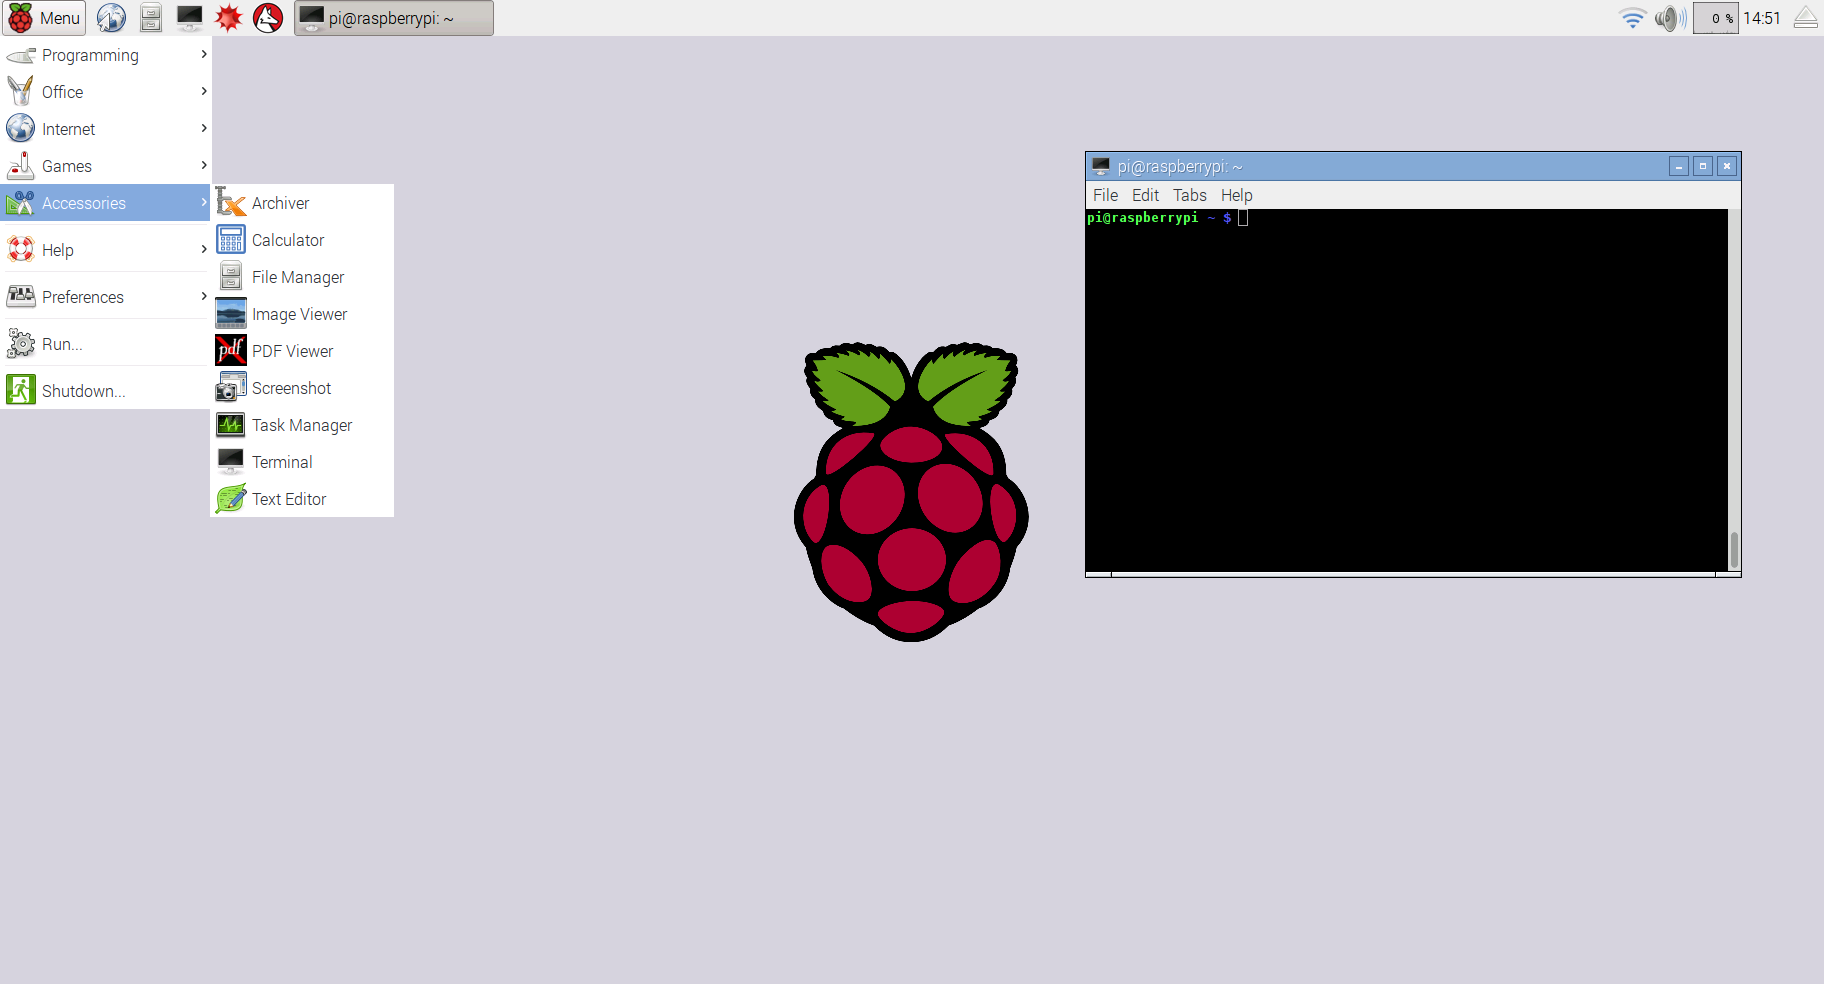
\includegraphics[scale=0.2]{raspbian}
    \caption{Raspbian Jessie with PIXEL Desktop environment}
  \end{center}
\end{figure}

\subsection{OpenCV Python Library}
Python is a general purpose programming language,. It became very popular in short time mainly because of its simplicity and code readability. 
It enables us to write our programs in fewer lines of code without reducing any readability.

With the support of Numpy python library, the task is easier. Numpy is a library that is optimized for numerical operations. In our code all 
OpenCV arrays are converted to the Numpy arrays. So we can do operations that we are able to do in Numpy arrays.

We decided to choose OpenCV python interface for fast prototyping and it has wide range for use cases. 
\begin{figure}[h!]
  \begin{center}
    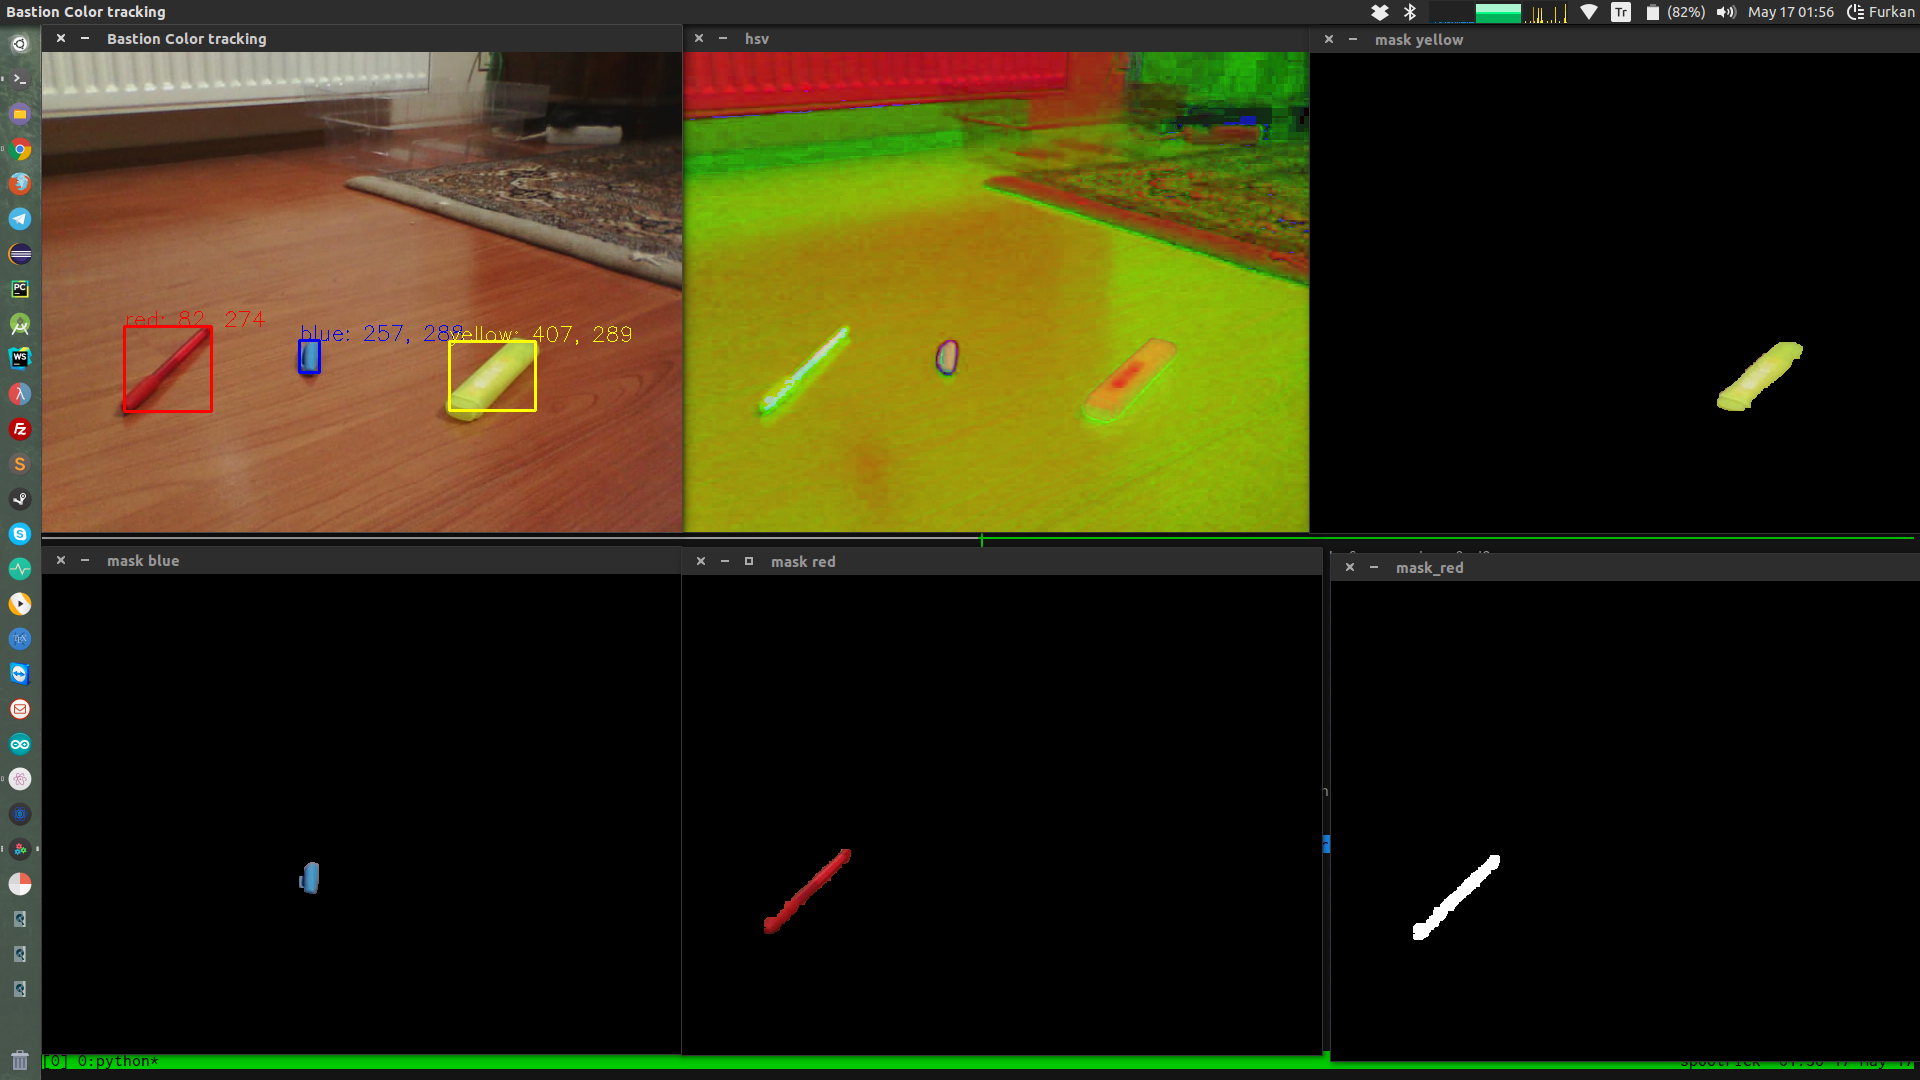
\includegraphics[scale=0.2]{opencv_python}
    \caption{OpenCV color detection and tracking}
  \end{center}
\end{figure}

\subsection{Serial Connection}
Controlling Arduino with WiFi is both unnecessary work and inefficient for us. That means extra WiFi module for Arduino, 
using pins for the module and ending up with less pins for other elements.

Raspberry Pi 3 comes with a built-in WiFi module. This means we can control Raspberry Pi 3 with WiFi. To make this control 
and connection easier, we control Arduino with Raspberry Pi 3. Raspberry Pi 3 is a small sized computer with full functionality, 
so when it connected to a Arduino, it can control the Arduino.

Both Raspberry Pi 3 and Arduino could be used to control the Bastion the Sentinel, but to get rid of the excess work, 
we constructed a master-slave relation between Raspberry Pi 3 and Arduino. 

Arduino controls Bastion the Sentinel via Serial Connection. Serial Connection is a kind of terminal to execute the codes in 
the Arduino microcontroller. A code/code block binded to a key, when a user pressed the designated key, Arduino IDE executes the code 
responding to the key.

Arduino serial communication runs on Raspberry Pi 3. We are controlling the Bastion the Sentinel and Arduino via Raspberry Pi 3’s WiFi.

When establishing connection via WiFi, connection security is a sensitive subject. We are establishing the security of the connection via 
Secure Shell (SSH). Secure Shell (SSH) basically a cryptographic network protocol. We are choosing to use it over an unsecured network 
connection. SSH provides a secure channel.

The way we follow to control the robot with serial connection is as follows:
\begin{itemize}
 \item Upload \verb|bastion.ino| arduino sketch to the Arduino Mega.
 \item Transfer \verb|bastion_serial_connection.py| python script to the Raspberry Pi.
 \item Control the robot with a laptop or with a smartphone.
\end{itemize}

\begin{figure}[h!]
  \begin{center}
    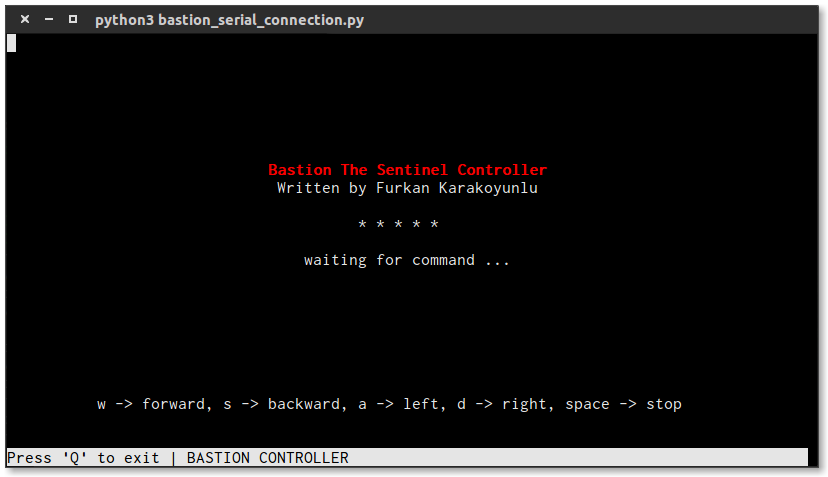
\includegraphics[scale=0.5]{serial_pc}
    \caption{Serial connection window from PC}
  \end{center}
\end{figure}

\begin{figure}[h!]
  \begin{center}
    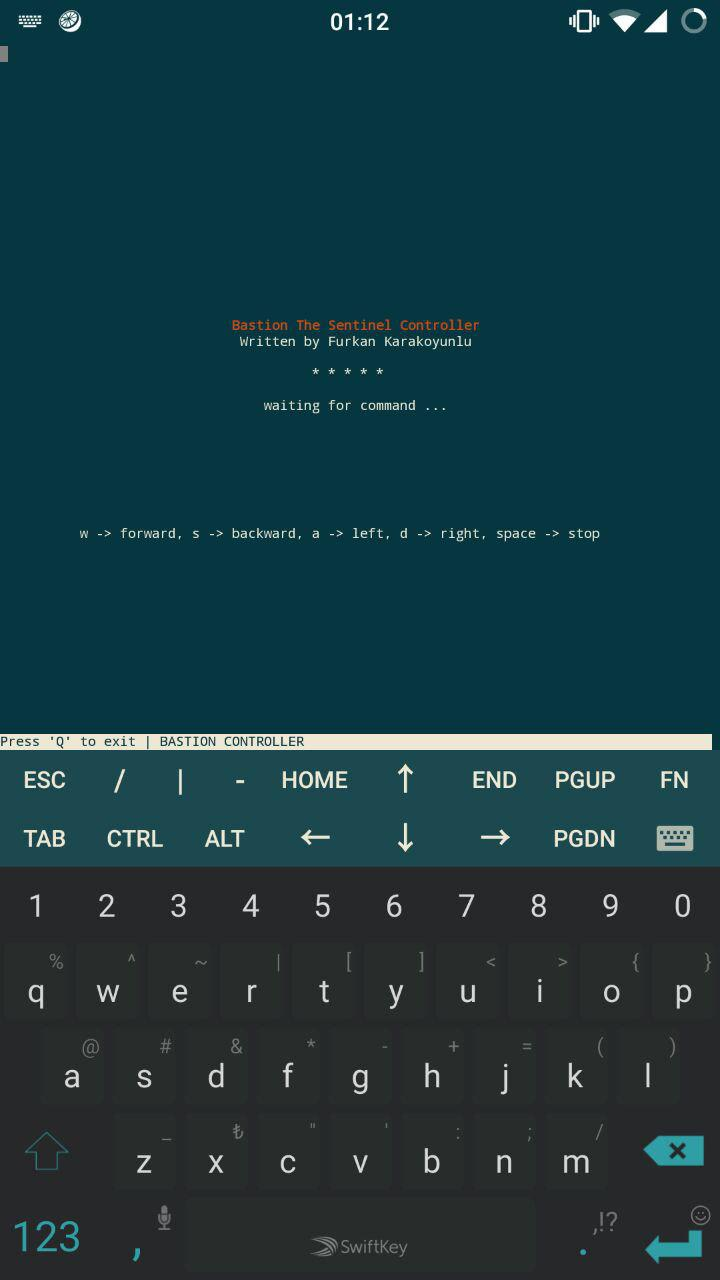
\includegraphics[scale=0.2]{serial_phone}
    \caption{Serial connection window from smartphone}
  \end{center}
\end{figure}




\pagebreak
\section{Source Codes}
All codes are available on \href {https://github.com/spootrick/Bastion}{https://github.com/spootrick/Bastion}\\

\bigskip
\verb|stream.py|: This python script basically gathers the video data on Raspberry Pi 3 and serves that data to http. 
It uses \verb|socketserver| and \verb|http| libraries to serve data and \verb|picamera| for gathering video data from 
Raspberry Pi camera module. This script runs on Raspberry Pi 3.
\begin{verbatim}
# ====================================
# -*- coding: utf-8 -*-
# project name:     Bastion The Sentinel
# file name:        stream.py
# python version:   3.4
# description:      Serve video data on http over the wifi
# ====================================

import io
import picamera
import logging
import socketserver
from threading import Condition
from http import server

PAGE="""
<!DOCTYPE html>
<html lang="en">
  <head>
    <meta charset="utf-8">
    <meta http-equiv="X-UA-Compatible" content="IE=edge">
    <meta name="viewport" content="width=device-width, initial-scale=1">
    <title>Bastion The Sentinel | Live Stream</title>
    <link rel="stylesheet" href="https://maxcdn.bootstrapcdn.com/bootstrap/3.3.7/css/bootstrap.min.css" integrity="sha384-BVYiiSIFeK1dGmJRAkycuHAHRg32OmUcww7on3RYdg4Va+PmSTsz/K68vbdEjh4u" crossorigin="anonymous">
    <link rel="stylesheet" href="https://maxcdn.bootstrapcdn.com/bootstrap/3.3.7/css/bootstrap-theme.min.css" integrity="sha384-rHyoN1iRsVXV4nD0JutlnGaslCJuC7uwjduW9SVrLvRYooPp2bWYgmgJQIXwl/Sp" crossorigin="anonymous">
    <!--[if lt IE 9]>
      <script src="https://oss.maxcdn.com/html5shiv/3.7.3/html5shiv.min.js"></script>
      <script src="https://oss.maxcdn.com/respond/1.4.2/respond.min.js"></script>
    <![endif]-->
  </head>
  <body>
    <div class="container">
      <div class="row">
        <div class="col-md-12 text-center">
          <h1><strong>Bastion The Sentinel</strong> Live Stream</h1>
          <img src="stream.mjpg" width="640" height="480" />
          <p>Live streaming from Bastion's Raspberry Pi 3.</p>
        </div>
      </div>
    </div>
  </body>
</html>
"""

class StreamingOutput(object):
    def __init__(self):
        self.frame = None
        self.buffer = io.BytesIO()
        self.condition = Condition()

    def write(self, buf):
        if buf.startswith(b'\xff\xd8'):
            # New frame, copy the existing buffer's content and notify all
            # clients it's available
            self.buffer.truncate()
            with self.condition:
                self.frame = self.buffer.getvalue()
                self.condition.notify_all()
            self.buffer.seek(0)
        return self.buffer.write(buf)

class StreamingHandler(server.BaseHTTPRequestHandler):
    def do_GET(self):
        if self.path == '/':
            self.send_response(301)
            self.send_header('Location', '/index.html')
            self.end_headers()
        elif self.path == '/index.html':
            content = PAGE.encode('utf-8')
            self.send_response(200)
            self.send_header('Content-Type', 'text/html')
            self.send_header('Content-Length', len(content))
            self.end_headers()
            self.wfile.write(content)
        elif self.path == '/stream.mjpg':
            self.send_response(200)
            self.send_header('Age', 0)
            self.send_header('Cache-Control', 'no-cache, private')
            self.send_header('Pragma', 'no-cache')
            self.send_header('Content-Type', 'multipart/x-mixed-replace; boundary=FRAME')
            self.end_headers()
            try:
                while True:
                    with output.condition:
                        output.condition.wait()
                        frame = output.frame
                    self.wfile.write(b'--FRAME\r\n')
                    self.send_header('Content-Type', 'image/jpeg')
                    self.send_header('Content-Length', len(frame))
                    self.end_headers()
                    self.wfile.write(frame)
                    self.wfile.write(b'\r\n')
            except Exception as e:
                logging.warning(
                    'Removed streaming client %s: %s',
                    self.client_address, str(e))
        else:
            self.send_error(404)
            self.end_headers()

class StreamingServer(socketserver.ThreadingMixIn, server.HTTPServer):
    allow_reuse_address = True
    daemon_threads = True

with picamera.PiCamera(resolution='640x480', framerate=12) as camera:
    output = StreamingOutput()
    camera.vflip = True
    camera.hflip = True
    camera.start_recording(output, format='mjpeg')
    try:
        address = ('', 8000)
        server = StreamingServer(address, StreamingHandler)
        server.serve_forever()
    finally:
        camera.stop_recording()
\end{verbatim}
\pagebreak
\verb|colorTracking.py|: This script detects and tracks the colors at the same time in given video file. Currently it will detect red, 
blue and yellow. It will read the named pipe.
\begin{verbatim}
# ====================================
# -*- coding: utf-8 -*-
# project name:     Bastion The Sentinel
# file name:        colorTracking.py
# python version:   3.4
# description:      tracking multiple colors at the same time with
#                   raspberry pi camera module with opencv python
#                   library
# ====================================

# importing libraries
try:
    import cv2
except ImportError:
    raise ImportError('Could not import cv2 library')

try:
    import numpy as np
except ImportError:
    raise ImportError('Could not import numpy library')


# capturing through named pipe
cap = cv2.VideoCapture(r'fifo264')

while 1:
    _, img = cap.read()

    # converting frame(img, i.e BGR) to HSV
    hsv = cv2.cvtColor(img, cv2.COLOR_BGR2HSV)

    # defining the range of red
    red_lower = np.array([136, 87, 111], np.uint8)
    red_upper = np.array([180, 255, 255], np.uint8)

    # defining the range of blue
    blue_lower = np.array([99, 115, 150], np.uint8)
    blue_upper = np.array([110, 255, 255], np.uint8)

    # defining the range of yellow
    yellow_lower = np.array([22, 60, 200], np.uint8)
    yellow_upper = np.array([60, 255, 255], np.uint8)

    # finding the range of red, blue and yellow in image
    red = cv2.inRange(hsv, red_lower, red_upper)
    blue = cv2.inRange(hsv, blue_lower, blue_upper)
    yellow = cv2.inRange(hsv, yellow_lower, yellow_upper)

    # Morphological transformation, Dilation
    kernal = np.ones((5, 5), "uint8")

    red = cv2.dilate(red, kernal)
    res_0 = cv2.bitwise_and(img, img, mask = red)

    blue = cv2.dilate(blue, kernal)
    res_1 = cv2.bitwise_and(img, img, mask = blue)

    yellow = cv2.dilate(yellow, kernal)
    res_2 = cv2.bitwise_and(img, img, mask = yellow)

    # Tracking the RED color
    (_, contours, hierarchy) = cv2.findContours(red, cv2.RETR_TREE, 
                                                    cv2.CHAIN_APPROX_SIMPLE)

    for pic, contour in enumerate(contours):
        area = cv2.contourArea(contour)
        if (area > 300):
            x, y, w, h = cv2.boundingRect(contour)
            img = cv2.rectangle(img, (x, y), (x + w, y + h), 
                                                       (0, 0, 255), 2)
            label_red = "red: {}, {}".format(x, y)
            cv2.putText(img, label_red, (x, y), cv2.FONT_HERSHEY_SIMPLEX, 
                                                          0.7, (0, 0, 255))

    # Tracking the BLUE color
    (_, contours, hierarchy) = cv2.findContours(blue, cv2.RETR_TREE, 
                                                    cv2.CHAIN_APPROX_SIMPLE)

    for pic, contour in enumerate(contours):
        area = cv2.contourArea(contour)
        if (area > 300):
            x, y, w, h = cv2.boundingRect(contour)
            img = cv2.rectangle(img, (x, y), (x + w, y + h), 
                                                           (255, 0, 0), 2)
            label_blue = "blue: {}, {}".format(x, y)
            cv2.putText(img, label_blue, (x, y), 
                                cv2.FONT_HERSHEY_SIMPLEX, 0.7, (255, 0, 0))

    # Tracking the YELLOW color
    (_, contours, hierarchy) = cv2.findContours(yellow, 
                                    cv2.RETR_TREE, cv2.CHAIN_APPROX_SIMPLE)

    for pic, contour in enumerate(contours):
        area = cv2.contourArea(contour)
        if (area > 300):
            x, y, w, h = cv2.boundingRect(contour)
            img = cv2.rectangle(img, (x, y), (x + w, y + h),
                                                         (0, 255, 255), 2)
            label_yellow = "yellow: {}, {}".format(x, y)
            cv2.putText(img, label_yellow, (x, y), 
                             cv2.FONT_HERSHEY_SIMPLEX, 0.7, (0, 255, 255))


    # show main window
    cv2.imshow("Bastion Color tracking", img)

    # show red mask window
    cv2.imshow("mask_red", red)
    # show red mask
    cv2.imshow("mask red", res_0)

    # show blue mask window
    cv2.imshow("mask blue", res_1)
    # show blue mask
    # cv2.imshow("mask_blue", blue)

    # show yellow mask window
    cv2.imshow("mask yellow", res_2)
    # show yellow mask
    # cv2.imshow("mask_yellow", yellow)

    # show converted hsv image
    cv2.imshow("hsv", hsv)

    if cv2.waitKey(10) & 0xFF == ord('q'):
        cap.release()
        cv2.destroyAllWindows()
        break
\end{verbatim}
\pagebreak
\verb|bastion.ino|: This is an arduino sketch which includes all motor controls and serial connection implementation.
\begin{verbatim}
#include "DualVNH5019MotorShield.h"

DualVNH5019MotorShield motorDriver;

/**
 * This method runs if there is a motor fault
 * and prints feedback to the serial.
 */
void stopIfFault(){
  if (motorDriver.getM1Fault()){
    Serial.println("M1 fault");
    while(1);
  }
  if (motorDriver.getM2Fault()){
    Serial.println("M2 fault");
    while(1);
  }
}


/**
 * Setup code which runs once.
 */
void setup() {
  Serial.begin(9600);
  Serial.setTimeout(50); // limiting the max wait time for serial data
  Serial.println("Serial connection established.");
  motorDriver.init();
}


/**
 * This method is for used to move the robot back and forth
 */
void setMotorSpeed(int speed){
  if(speed >= -400 && speed <= 400){
    motorDriver.setM1Speed(speed);
    motorDriver.setM2Speed(speed);

    stopIfFault();
    delay(1);
  }
}


/**
 * This method is for turning left
 */
void turnLeft(){
  motorDriver.setM1Speed(100);
  motorDriver.setM2Speed(-100);
  delay(225);
  motorDriver.setM1Speed(0);
  motorDriver.setM2Speed(0);
}


/**
 * This method is for turning right
 */
void turnRight(){
  motorDriver.setM1Speed(-100);
  motorDriver.setM2Speed(100);
  delay(225);
  motorDriver.setM1Speed(0);
  motorDriver.setM2Speed(0);
}

/**
 * Main code which runs repeatedly
 */
void loop() {
  if(Serial.available()){
    switch(Serial.parseInt()){
      case 0: // stop
        setMotorSpeed(0);
        break;
      case 1: // move forward 200
        setMotorSpeed(200);
        break;
      case 2: // move backward 200
        setMotorSpeed(-200);
        break;
      case 3: // move forward 400
        setMotorSpeed(400);
        break;
      case 4: // move backward 400
        setMotorSpeed(-400);
        break;
      case 5: // turn left
        turnLeft();
        break;
      case 6: // turn right
        turnRight();
        break;
      default:
        Serial.println("Uups!.. Wrong command entered!");
    }
  }
  delay(1);
}
\end{verbatim}
\pagebreak
\verb|bastion_serial_connection.py|: This python script is used by Raspberry Pi to control the serial 
connection on Arduino. This script can be easily used all devices (PC, smartphone, etc.) which can make ssh connections to the
Raspberry Pi.
\begin{verbatim}
#!/usr/bin/env python
# -- coding: utf-8 --
# File              : bastion.py
# Description       : Serial connection script for arduino
# Author            : Furkan Karakoyunlu
# Date              : 21.05.2017
# Python version    : 3.4
# =======================================

import sys,os

try:
    import curses
except ImportError:
    raise ImportError("The library 'curses' couldn't imported")

try:
    import serial
except ImportError:
    raise ImportError("The library 'serial' couldn't imported")


def draw_screen_for_serial_connection(screen):
    # do not echo keys to the screen
    curses.noecho()
    # send keys without pressing enter
    curses.cbreak()

    try:
      serial_connection = serial.Serial('/dev/ttyACM0', 9600)
    except:
      print('Error: Cannot connected to the arduino!')
      sys.exit()

    command = ''
    k = 0

    cursor_x = 0
    cursor_y = 0

    # starting colors for curses
    curses.start_color()
    curses.init_pair(1, curses.COLOR_RED, curses.COLOR_BLACK)
    curses.init_pair(2, curses.COLOR_BLACK, curses.COLOR_WHITE)

    # looping the last pressed key k
    while (k != ord('Q')):
        # initialization
        screen.clear()
        height, width = screen.getmaxyx()

        if k == ord('w'): # forward 200
            serial_connection.write(bytes('1', 'UTF-8'))
            command = 'FORWARD 200'
        elif k == ord('s'): # backward 200
            serial_connection.write(bytes('2', 'UTF-8'))
            command = 'BACKWARD 200'
        if k == ord('W'): # forward 400
            serial_connection.write(bytes('3', 'UTF-8'))
            command = 'FORWARD 400'
        elif k == ord('S'): # backward 400
            serial_connection.write(bytes('4', 'UTF-8'))
            command = 'BACKWARD 400'
        elif k == ord('a'): # turn left
            serial_connection.write(bytes('5', 'UTF-8'))
            command = 'TURN LEFT'
        elif k == ord('d'): # turn right
            serial_connection.write(bytes('6', 'UTF-8'))
            command = 'TURN RIGHT'
        elif k == ord(' '): # stop
            serial_connection.write(bytes('0', 'UTF-8'))
            command = 'STOP'

        # declare the strings
        title = "Bastion The Sentinel Controller"[:width-1]
        subtitle = "Written by spootrick"[:width-1]
        keystr = "Last command: {}".format(command)[:width-1]
        helpstr = "w -> forward, s -> backward, a -> left, d -> right, 
                                                              space -> stop"
        statusbarstr = "Press 'Q' to exit | BASTION CONTROLLER"

        if command == '':
            keystr = "waiting for command ..."[:width-1]

        # text centering
        start_x_title = int((width // 2) - (len(title) // 2) - len(title) % 2)
        start_x_subtitle = int((width // 2) - (len(subtitle) // 2) 
                                                          - len(subtitle) % 2)
                                                          
        start_x_keystr = int((width // 2) - (len(keystr) // 2) 
                                                            - len(keystr) % 2)
        start_y = int((height // 2) - 5)

        # render status bar
        screen.attron(curses.color_pair(2))
        screen.addstr(height-1, 0, statusbarstr)
        screen.addstr(height-1, len(statusbarstr), " " * (width
                                                    - len(statusbarstr) - 1))
        screen.attroff(curses.color_pair(2))

        # turning on attributes for title
        screen.attron(curses.color_pair(1))
        screen.attron(curses.A_BOLD)

        # render title
        screen.addstr(start_y, start_x_title, title)

        # turning off attributes for title
        screen.attroff(curses.color_pair(1))
        screen.attroff(curses.A_BOLD)

        # printing the rest of the text
        screen.addstr(start_y + 1, start_x_subtitle, subtitle)
        screen.addstr(start_y + 3, (width // 2) - 6, '* * * * *')
        screen.addstr(start_y + 5, start_x_keystr, keystr)
        screen.addstr(start_y + 13, (width // 2) - 35 , helpstr)
        screen.move(cursor_y, cursor_x)

        # refresh screen
        screen.refresh()

        # wait for next input
        k = screen.getch()

def main():
    curses.wrapper(draw_screen_for_serial_connection)

if __name__ == "__main__":
    main()
\end{verbatim}


\pagebreak
\section{References}
\begin{itemize}
 \item \href{https://www.pololu.com/product/2502}{https://www.pololu.com/product/2502}
 \item \href{https://www.pololu.com/file/download/vnh5019.pdf?file_id=0J504}{https://www.pololu.com/file/download/vnh5019.pdf?file\_id=0J504}
 \item \href{https://www.raspberrypi.org/}{https://www.raspberrypi.org/}
 \item \href{http://opencv.org/}{http://opencv.org/}
 \item \href{https://picamera.readthedocs.io/en/release-1.13/recipes2.html#web-streaming}{https://picamera.readthedocs.io/en/release-1.13/recipes2.html\#web-streaming}
 \item \href{https://www.digitalocean.com/community/tutorials/how-to-use-netcat-to-establish-and-test-tcp-and-udp-connections-on-a-vps}{https://www.digitalocean.com/community/tutorials/how-to-use-netcat-to-establish-and-test-tcp-and-udp-connections-on-a-vps}
 \item \href{http://www.tldp.org/LDP/lpg/node15.html}{http://www.tldp.org/LDP/lpg/node15.html}
 \item \href{https://docs.python.org/3/howto/curses.html}{https://docs.python.org/3/howto/curses.html}
 
\end{itemize}



\end{document}

